\documentclass{llncs}

\usepackage{amssymb}
\setcounter{tocdepth}{3}
\usepackage{graphicx}
\usepackage[table,xcdraw]{xcolor}
\usepackage[ruled]{algorithm2e}
%\usepackage[lined,boxed,commentsnumbered]{algorithm2e}
\usepackage{amssymb}
\usepackage{amsmath,graphicx,color,doi}
\usepackage{algorithm2e}
%\usepackage{algorithmic}	
\usepackage{multirow}
\usepackage{subfigure}
\usepackage{cite}


\newcommand{\gi}[1]{{\textcolor{red}{[\small \textbf{Giacomo}: #1]}}}
\newcommand{\ad}[1]{{\textcolor{red}{[\small \textbf{Adriano}: #1]}}}
\newcommand{\cl}[1]{{\textcolor{red}{[\small \textbf{Claudio}: #1]}}}

%\newcommand{\gi}[1]{}
%\newcommand{\ad}[1]{}
%\newcommand{\cl}[1]{}


\begin{document}
\title{Tampering Detection In Low-Power Smart Cameras}

\author{Adriano Gaibotti\inst{1} \and Claudio Marchisio\inst{1} \and Alexandro Sentinelli\inst{1} \and Giacomo Boracchi\inst{2}}

\institute{ 
	STMicroelectronics, Advanced System Technology, Via Camillo Olivetti 2, 20864, Agrate Brianza (MB), Italy\\
	\email{\{adriano.gaibotti, claudio.marchisio, alexandro.sentinelli\}@st.com}
	\and
	Politecnico di Milano, Dipartimento di Elettronica, Informazione e Bioingegneria (DEIB), Via Ponzio 34/5, 20133, Milano (MI), Italy\\
	\email{giacomo.boracchi@polimi.it}
}
\maketitle

\begin{abstract}
A desirable feature for smart cameras is the ability to autonomously detect any tampering event/attack that would prevent a clear view over the monitored scene. No matter whether tampering is due to atmospheric phenomena (e.g., few rain drops over the camera lens) or to malicious attacks (e.g., the device displacement), these have to be promptly detected to possibly activate countermeasures. Tampering detection becomes particularly challenging in battery-powered cameras, where it is not possible to acquire images at video-like frame-rates, nor use sophisticated image-analysis algorithms. 

We here introduce a tampering-detection algorithm that has been specifically designed for low-power smart cameras: the algorithm leverages very simple indicators that are then monitored by an outlier-detection scheme. Any frame yielding anomalous indicator is detected as a tampering attempt. Core of the algorithm is the partitioning of the scene into adaptively defined regions, that are preliminarily defined by segmenting the image during the algorithm-configuration phase, and which shows to substantially improve the detection of camera displacements. Our experiments show that the proposed algorithm can successfully operate on sequences acquired at very low-frame rate, such as one frame every minute, and at a very small computational complexity. %and leveraging the image partitioning into regions yields improved performance with respect to monitoring the whole scene


\keywords{tampering detection, defocus, displacement detection}
\end{abstract}



\section{Introduction}\label{sec:introduction}
%\gi{Adriano: decidi che email tenere, non tutte e due :)}

%We here address the problem of detecting tampering events/attacks in camera devices, and in particular those preventing the proper acquisition of the monitored scene. 

% What is the problem?
When cameras operate outdoor and in harsh environments, dust, rain drops or snow flakes might lie on the camera lens resulting in blurry pictures, as in Fig. \ref{fig:pioggia}, or in partial occlusions of the scene, as in Fig. \ref{fig:neve}. Similarly, intentional attacks like displacing the camera, changing its focus, or spraying some opaque or glossy liquid over the lenses, would result in heavily compromised pictures, that would be surely useless for monitoring purposes. We refer to these events/attacks as tampering. In some cases, tampering is easy to detect, e.g., when the camera integrity is affected and the device goes out-of-order. However, in many other situations, namely when the device is not physically damaged, tampering detection is not straightforward, and sometimes image analysis is the only viable option. 

% Why is it interesting and important?
Tampering prevents the correct scene interpretation and causes the loss of small, important details such as licence plates. Tampering detection is therefore an essential feature in surveillance systems~\cite{hampapur2005smart}, where cameras are expected to autonomously detect any tampering, and promptly reporting alerts. Surveillance cameras are typically connected to the power supply and operates at normal frame-rates (e.g. around few frames per second): in these conditions, several tampering-detection algorithms have been presented~\gi{Adriano add REFERENCES}.  

\gi{Qui ST pu\'o aggiungere qualche esempio di applicazione qui o menzionare dispositivi di riferimento (con tanto di link a datasheet). Magari aggiungendo che le batterie recenti permettono operativit\'a di due anni a questi regimi.}\cl{Verifico cosa possiamo dire del SecSoc.}
%
In this work we expressly target low-power and ultra-low-power smart cameras, devices that operate at very low frame-rates (e.g. possibly less than one frame every minute), that are characterized by a constrained computational power and memory, and that are battery powered (typically lasting one or two years). As an example, consider Wireless Multimedia Sensor Networks (WMSN) \cite{akyildiz2007survey} where nodes are wirelessy connected smart-cameras, that can acquire and transmit images at regular time interval or upon requests. Often, in WMSN, the units are not connected to the power supply and have to operate with batteries and possibly rely on energy harvesting mechanisms~\gi{REFERENCES, Adriano, guarda se c'e' qualche reference dal nostro paper di TIM} \cite{magno2009adaptive}. Therefore, the power consumption is a serious concern in these devices.

Even though low-power and ultra-low-power cameras not employed in critical surveillance applications, these devices are becoming popular in distributed systems for monitoring wide environments due to their low cost and maintenance requirements \gi{Adriano, Claudio, possiamo mettere qualche REFERENCE?}. Tampering detection is therefore very important in low-power smart cameras, where the algorithm are expected to be particularly prompt and have low false-alarm rates to prevent unnecessary energy-demanding operations like the local processing or radio activation for transmitting corrupted images (or false alarms) over the network. Unfortunately, tampering detection in such a resource-constrained scenario, has been much less investigated.

% Why is it hard? (E.g., why do naive approaches fail?)
Tampering detection in low-power smart cameras is much more challenging than in conventional surveillance cameras~\cite{perrig2004security}. Beside computational aspects -- such as the number of operations per pixels allowed -- the big issue is that low-power smart cameras typically operate at very low-frame rates (e.g., less than one frame per minute), thus the acquired sequence does not evolve smoothly. This prevents the use of learned background models and the analysis of foreground variations \cite{piccardi2004background}. When dynamic environments are acquired at low frame rates, two consecutive frames might be very different because of changes in the scene and in the light conditions, resulting in sequences those depicted in Figure~\ref{fig:sequences}: smart cameras have to correctly distinguish between these \emph{normal} changes and changes due to camera tampering. 

% We here address the problem of detecting tampering events on a camera device that is employed for monitoring purpose. Tampering events can be due to malicious attacks, as for instance a displacement of the camera or spraying some dirty liquid that would prevent the acquisition of (part of) the monitored scene or the interpretation of the content (e.g., the identification of licence plates). 

%What are the key components of my approach and results? Also include any specific limitations.
We present an algorithm to detect both camera defocus and displacement, as stated in Section \ref{sec:probForm}. The algorithm presented in Section~\ref{sec:propSol} relies on two indicators: the average image intensity to detect displacement, and the average gradient norm, to detect blur. These indicators can be easily computed and monitored by an outlier-detection technique to detect the respective tampering. We show that displacement-detection performance can be improved by means of a preliminarily partitioning of the scene into nonoverlapping regions, and then separately computing and monitoring the average intensity over different regions (Section \ref{subsec:Segmentation}). Remarkably, these regions need to be defined during an initial configuration phase of the smart camera, thus there is no relevant computational overhead w.r.t. monitoring the whole image. Experiments in Section \ref{sec:experiments} show that operating on image regions can substantially improve the detection of camera displacements. Concluding remarks and discussions are given in Section \ref{sec:Conclusion}.

\begin{figure}[t!]
\centering
\subfigure[]{\label{fig:pioggia} 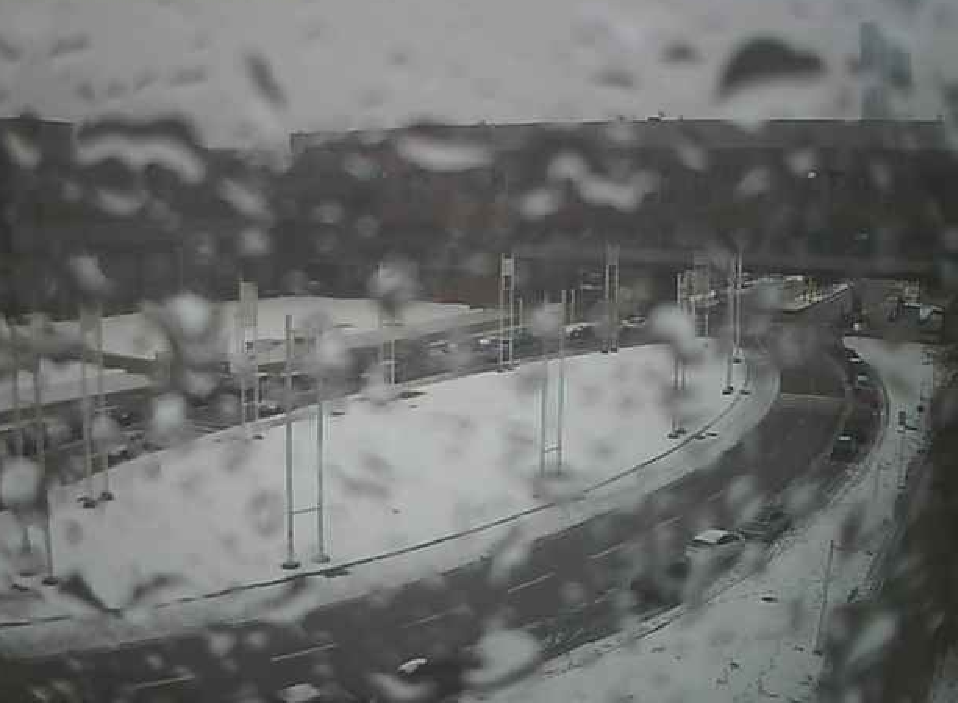
\includegraphics[width=0.4\linewidth]{Immagini/pioggia}}
\subfigure[]{\label{fig:neve} 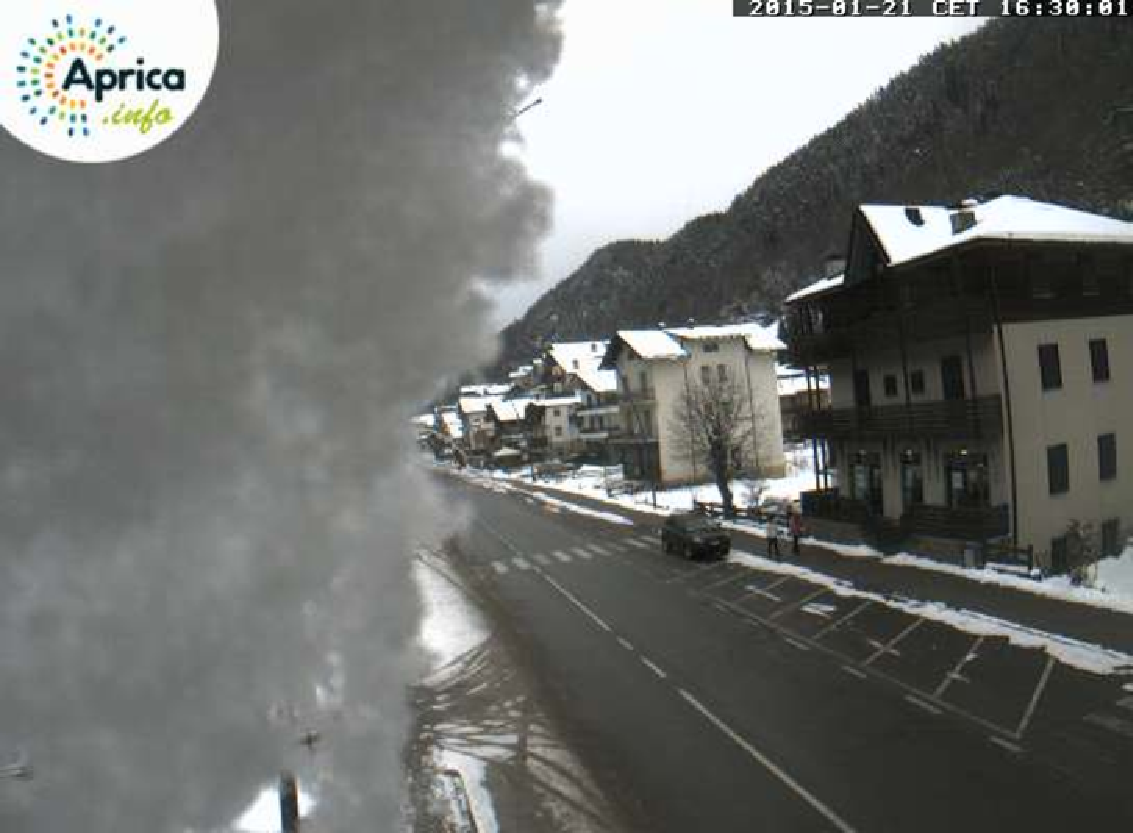
\includegraphics[width=0.4\linewidth]{Immagini/neve}}
\caption[Tampering examples]{Examples of tampering events due to atmospheric phenomena. \textbf{(a)} Blur due to rain drops on the camera lens. \textbf{(b)} Occlusion due to snow on the camera lens.}
\label{fig:tampering}
\end{figure}


\subsection{Related Works}\label{subsec:relWorks}
% Why hasn't it been solved before? (Or, what's wrong with previous proposed solutions? How does mine differ?)
The literature concerning tampering detection is mostly focused on video surveillance applications and operates at few frames per second \gi{Adriano, \'e vero?}. Background models are typically leveraged to identify defocus and occlusions; in particular~\cite{aksay2007camera} performs defocus detection by analyzing the wavelet domain of each frame and performs histogram comparison for detecting occlusions, while camera displacements are not considered. A background-subtraction technique is employed in~\cite{saglam2009real} to identify defocus, occlusions, and displacements. \gi{FIXME Comparison in the Fourier domain for defocus detection, histogram comparison for occlusion detection, comparison between current background and delayed background for displacement detection}. Background subtraction is also used in \cite{gil2007automatic} to detect defocus, occlusions, and displacements. \gi{FIXME Comparison of edges pixels count for defocus detection, entropy comparison for occlusion detection, block matching algorithm for displacement detection}.
In contrast, no background models are used in \cite{alippi2010detecting}, where a sequential monitoring scheme based on a change-detection test is employed to detect changes in the average gradient energy of each frame to detect defocus due to external disturbances on the camera lens.  
\cite{ribnick2006real}: comparison between frames belonging to a buffer in order to find high values of dissimilarity, associated to tampering.
\cite{kryjak2012fpga}: implementation in a FPGA of a solution based on background modeling, histograms comparisons, edges comparisons.
\cite{harasse2004automated}: tampering detection inside a moving vehicle; uses background subtraction methods in order to identify defocus, occlusions, and displacements. Comparison of edges pixels count for defocus detection, entropy comparison for occlusion detection, block matching algorithm for displacement detection.
\cite{tsesmelis2013tamper}: monitoring of the number of key points extracted by SURF in order to detect defocus events, partition in blocks and HOG descriptors matching for each block in order to detect occlusions. These types of solutions requires a lot of computations
%
%
%
\section{Problem Formulation}\label{sec:probForm}
%
Let $z_t$ be the frame acquired at time $t$, which we model as
\begin{equation}
\label{eq:observationModel}
z_t(x)=\mathcal{D}_t[y_t](x) \quad \forall x \in X
\end{equation}
where $\mathcal{D}_t$ denotes the degradation operator that transforms the original image $y_t$ in the frame $z_t$; $X \subset \mathbb{Z}^2$ denotes the regular pixels grid and $x\in \mathbb{Z}^2$ indicates the pixel coordinates. As far as there is no tampering attacks/events,
\begin{equation}
\label{eq:no_tampering}
\mathcal{D}_t[y_t](x) = y_t(x) + \eta_t(x) \quad \forall x \in X
\end{equation}
where $\eta_t$ is a random variable accounting for different noise sources (e.g., thermal, quantization, photon-counting). In normal conditions, all the images $y_t$ (thus also the frames $z_t$) might show different content but are acquired from the same viewpoint and the same camera orientation.

When at time $\tau^*$ an external disturbance introduces \emph{blur/defocus}, the image $y_t$ is degraded by a spatially variant blur operator, and $z_t$ becomes
\begin{equation}
\label{eq:model_defocus}
\mathcal{D}_t[y_t](x) = \int_{\mathcal{X}}y(s)h_t(x,s)ds\, + \eta_t(x) \quad \forall x \in X, t \geq \tau^*
\end{equation}
where $h_t(x,\cdot) > 0$ is the point-spread function at pixel $x \in X$.

A \emph{camera displacement} at frame $\tau^*$ is instead modeled as 
\begin{equation}
\label{eq:model_displacement}
z_t(x)  = \left\{ \begin{array}{rcl}
y_t(x) + \eta(x) & \mbox{per} & t < T^* \\
w_t(x) + \eta(x) & \mbox{per} & t \geqslant T^*
\end{array}\right. ,
\end{equation}
where $w_t$ relates to a different viewpoint and/or camera orientation than $y_t$. 

The proposed tampering-detection algorithm analyzes a sequence of frames $\{z_t\}_t$ to detect time $\tau^*$ when any tampering like \eqref{eq:model_defocus} or \eqref{eq:model_displacement} occurs. We require that the initial $T_0$ frames are without tampering and provided for training.


\section{The Proposed Algorithm}\label{sec:propSol}

Algorithm \ref{alg:DISPL} presents the proposed tampering detection, which relies on two indicators that are very simple to compute: the average intensity (also referred to as \emph{luma}, and denoted by $l$) and the average norm of the gradient (denoted by $g$). The former is meant to detect camera displacement, the latter camera defocus. As anticipated in Section \ref{sec:introduction}, during the initial configuration, the scene is segmented in $\{R_k\}, k = 1,\dots,K$ disjoint regions ($R_k \subset \mathcal{X}, R_i \cap R_j = \emptyset, \forall i \neq j$). Details about the employed segmentation algorithm are in Section \ref{subsec:Segmentation}. 

In each frame $z_t$ the luma is separately computed in of the $K$ regions,
\begin{equation}\label{eq:lumaRegions}
l_k(t) =\frac{1}{\#R_k} \sum_{R_k} z_t(x), \ \ k = 1, \dots, K\,,
\end{equation}
while the average gradient norm is computed over the whole image
\begin{equation}
\label{eq:normaGradiente}
g(t) = \sum_X \left (\sqrt{\left(z_t \circledast f_h\right)^2(x) + \left(z_t \circledast f_v\right)^2(x)}\right),
\end{equation}
where $f_h$ and $f_h$ are the horizontal and vertical derivative filters, respectively, $\#(\cdot)$ indicates the cardinality of a set and $\circledast$ the 2d convolution.

\begin{figure}[tb]
\centering
\label{fig:indicatori} 
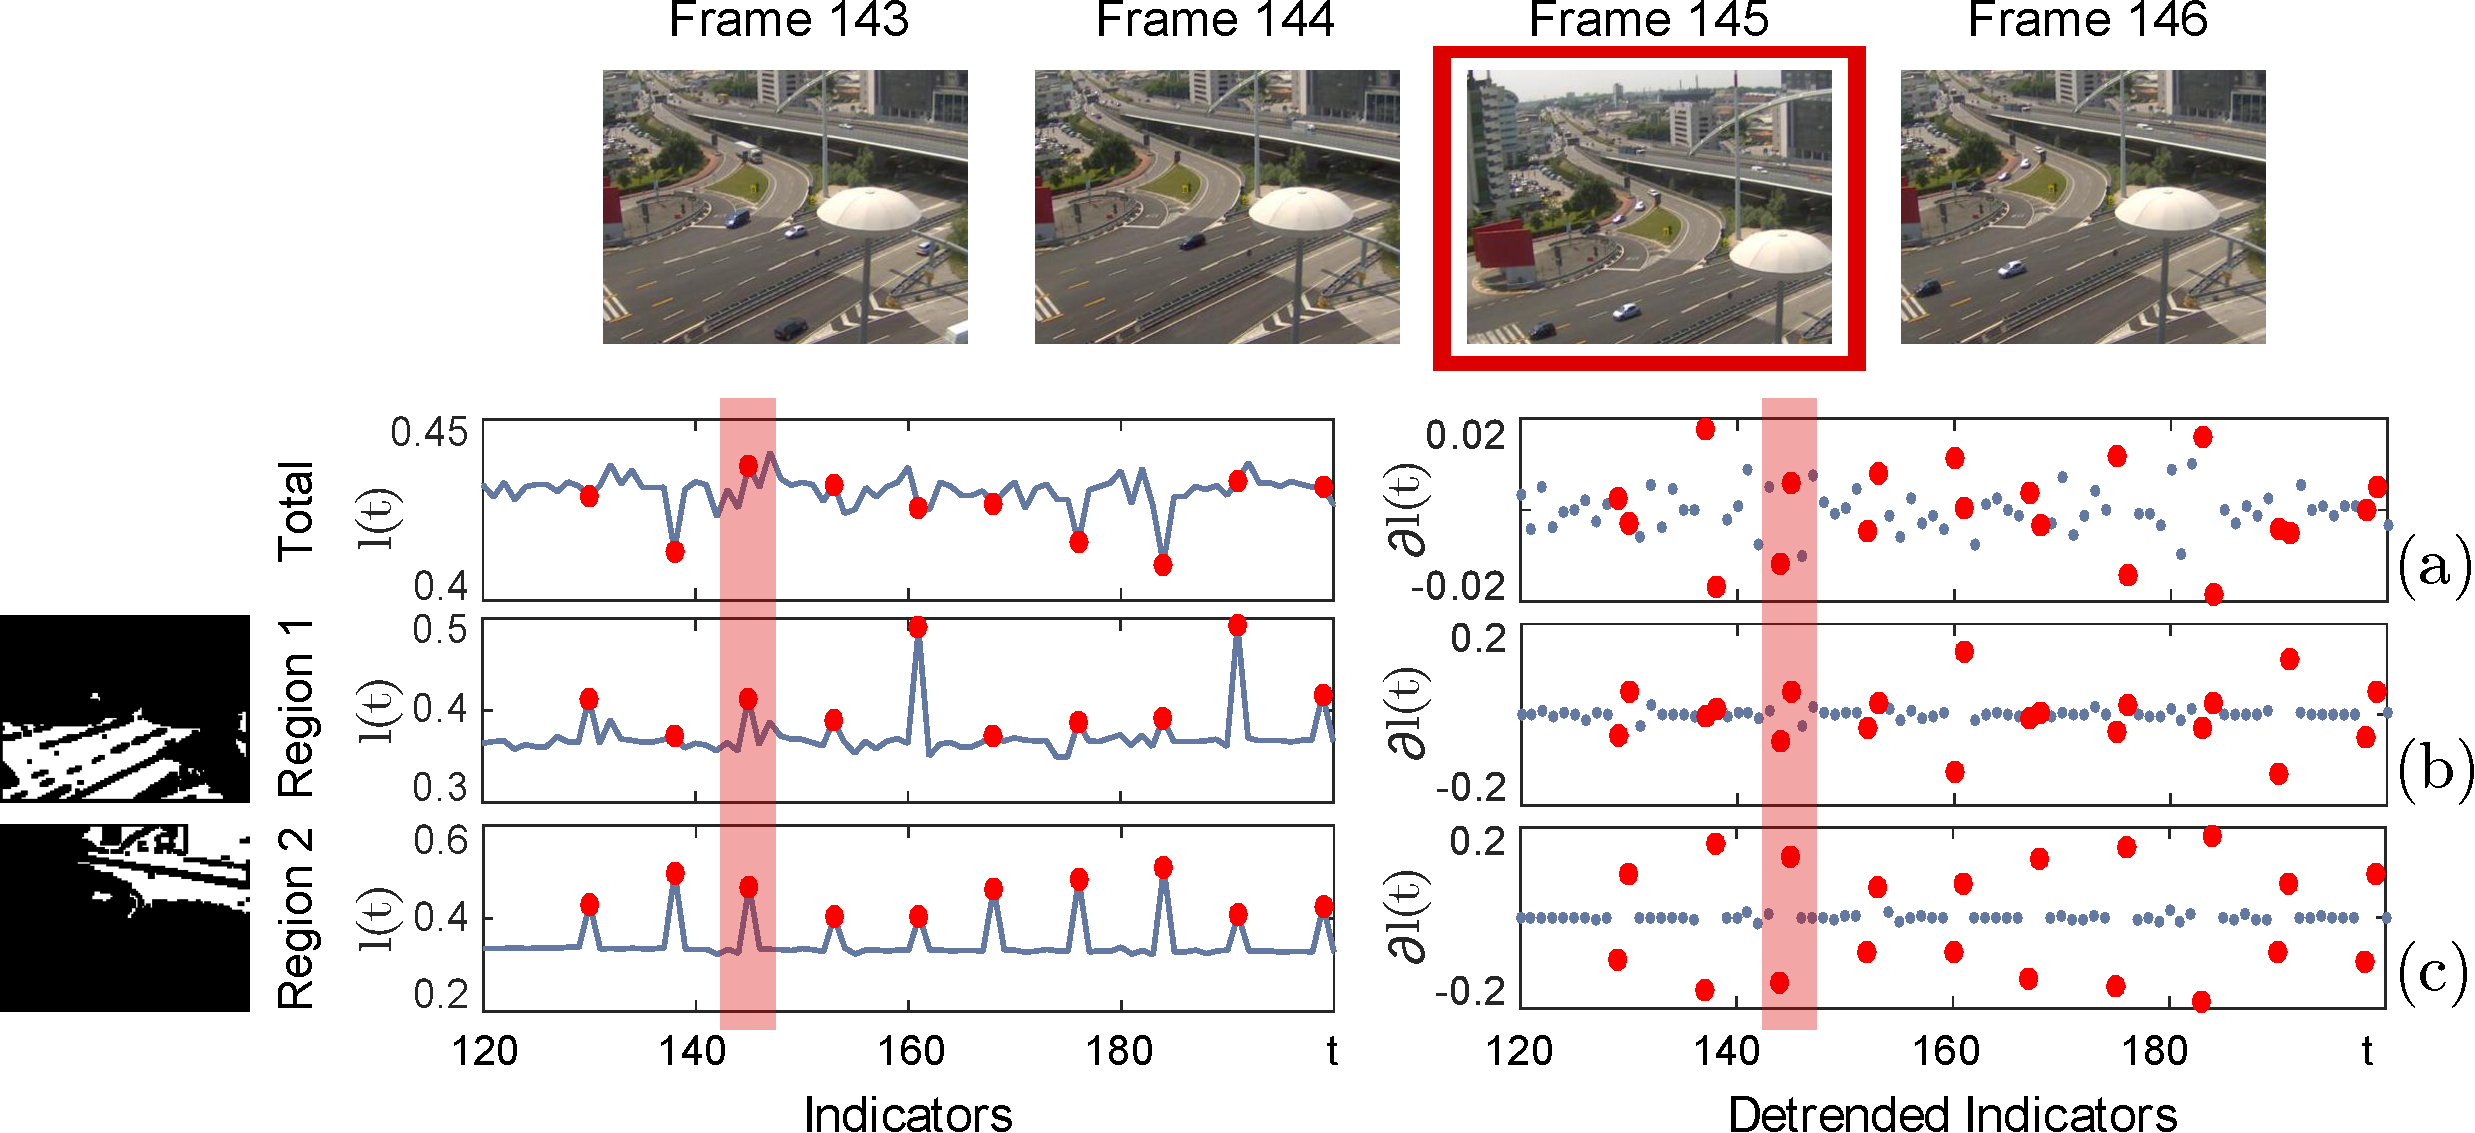
\includegraphics[width=1\linewidth]{Immagini/indicatori}
\caption{Behavior of the average norm of the gradient \textbf{(a)} and its detrending \textbf{(b)} in a sequence with a defocus event.
The tampering event come at $t = 600$.
As illustrated in \textbf{(a)}, even in the case in which there aren't tampering events, there is nonstationarity.
Detrending is done in order to preserve stationarity in normal situations.
Considering the detrending \textbf{(b)} persistent changes become instantaneous:
in particular there is a peak in the instant in which tampering begins.}
\end{figure}

As shown in Figure \ref{fig:indicatori}(a), tampering results in outliers in the sequence of indicators. Detecting these outliers is not straightforward, since indicators heavily fluctuates in normal conditions because of short-term variations in the depicted scene or illumination changes. For outlier-detection purposes~\cite{Chandola2009}, it is more convenient to operate on sequences of independent and identically distributed (i.i.d.) values, where outliers can be detected by density-based methods or simply by confidence regions that is what we considered in our algorithm. Unfortunately, trends or deterministic variations in the indicator sequences are not easy to compensate because of unpredictable evolutions of the scene. 

To obtain indicators that in normal conditions can be treated as i.i.d. realizations of a random variable we, detrend~\cite{Gustafsson2000} the indicator sequence by a temporal derivative
\begin{equation}\label{eq:detrending}
 \partial l_k(t) = l_k(t)-l_k(t-1),  \ \ k = 1, \dots, K\,,
\end{equation}
and we similarly define $\partial g(t)$. Detrended indicators are more suitable to be monitored by a confidence interval since, as shown in Figure \ref{fig:indicatori}(b). However, a tampering yielding permanent changes in the indicators, as those in Figure \ref{fig:indicatori}(a) results in a single outlier in the detrended indicator~\eqref{eq:detrending}. 


We perform outlier detection by defining confidence regions for our indicator in tampering-free frames. In practice, since all these are scalar indicators, it is enough to compute the indicator mean ($\overline{\partial l}_k(t), k = 1,\dots,K$ and $\overline{\partial g}(t)$) and standard deviations ($\sigma_{l_k}, k = 1,\dots,K$ and $\sigma_g$) over the tampering-free frames provided for training, namely $z_t\,, t = 1, \dots, T_o$. Confidence regions are then defined as 
\begin{equation}\label{eq:confidenceRegions}
 [\overline{\partial l}_k(t) - \gamma \sigma_{l_k}, \overline{\partial l}_k(t) + \gamma \sigma_{l_k}],  k = 1,\dots,K
\end{equation}
where $\gamma >0$ is a tuning parameter. A similar region is built for $\partial g$. During operations, any indicator falling outside the corresponding confidence region is considered anomalous and tampering is detected. 


\begin{algorithm}[t]
	% \SetAlgoNoLine
	\LinesNumbered
	\SetAlgoNlRelativeSize{0}
	\SetNlSty{small}{}{.}
	\textbf{Input}: $\gamma$, $T_{o}$, $\{R_k\} k=1,\dots,K$ \\
	\textbf{Configuration}:\\
	\lnl{DISPL-Tr1} Compute $\partial l_k(t)$ and $\partial g(t), t = 1, \cdots, T_o$\\ 
	\lnl{DISPL-Tr7} Compute $\sigma_{l_k}$ and $\sigma_{g}$, the standard deviations of $\partial l_k$ and $\partial g$.\\
	
	\textbf{Operational phase}:\\
	\lnl{DISPL-Test1} \For{$t=T_{o} + 1,\dots,\infty$}{
		\lnl{DISPL-Test2} Get frame $z_t$, set $n_l =0$
		\lnl{DISPL-Test4} \For{$k=1,\dots,K$}{
			\lnl{DISPL-Test5} Compute $\partial l_k(t)$\\
			\lnl{DISPL-Test6} \If{$\partial l_k(t) < -\gamma \sigma_{l_k} \vee \partial l_k(t) > \gamma \sigma_{l_k} $}{
				\lnl{DISPL-Test7} $n_l=n_l+1$\\
			}
		}
		\lnl{DISPL-Test8} \If{$n_l\geq K-1$}{
			\lnl{DISPL-Test9} tampering (probably displacement or occlusion) has occurred in $z_t$ \\
		}
		\lnl{DISPL-Test10} Compute $\partial g(t)$\\
		\lnl{DISPL-Test11} \If{$\partial g(t) < -\gamma \sigma_{g} \vee \partial l(t) > \gamma \sigma_{g} $}{
				\lnl{DISPL-Test9} tampering (probably out-of-focus) has occurred in $z_t$ \\
								}
	}   
	\caption{The Proposed Tampering-Detection Algorithm}
	\label{alg:DISPL}
\end{algorithm}

\subsection{Scene Segmentation}\label{subsec:Segmentation}
Consideriamo la sequenza $\{z_t\}$ di frame acquisiti dalla camera, con $t=1,\dots,T_{c}$.
Per ciascun pixel $x\in\mathcal{X}$ calcoliamo un vettore $\textbf{d}(x)$ di $5$ elementi
\begin{equation}
\label{eq:featureVector}
\textbf{d}(x)=\left[r(x);c(x);\mu_{\nabla}(x);\sigma_{\nabla}(x);\bar{z}(x)\right], \textbf{d}(x) \in \mathbb{R}^5
\end{equation}
dove:
\begin{itemize}
	\item $r(x)$ rappresenta il numero di riga del pixel $x$.
	\item $c(x)$ rappresenta il numero di colonna del pixel $x$.
	\item $\mu_{\nabla}(x)$ rappresenta il valore del gradiente nel pixel $x$ mediato nel tempo:
	\begin{equation}
	\label{eq:segmentazioneGrad}
	\mu_{\nabla}(x) = \frac{\sum_{t=1}^{T_c}(\|\nabla z_t\|_2^2 \circledast f)(x)}{T_c},
	\end{equation}
	dove abbiamo indicato con $\|\nabla z_t\|_2^2$ la norma del gradiente per l'immagine $z_t$, definita in \eqref{eq:normaGradiente}, e con $f$ il filtro gaussiano discreto derivato dal campionamento di \eqref{eq:gaussian}.
	\item $\sigma_{\nabla}(x)$ rappresenta la deviazione standard nel tempo del gradiente nel pixel $x$:
	\begin{equation}
	\label{eq:segmentazioneVar}
	\sigma_{\nabla}(x)=\sqrt{\frac{1}{T_c - 1}\sum_{t=1}^{T_c}\left(\left(\|\nabla z_t\|_2^2 \circledast f\right)(x)-\mu_{\nabla}(x)\right)^2}.
	\end{equation}
	\item $\bar{z}(x)$ rappresenta il valore della luma del pixel $x$ mediato nel tempo:
	\begin{equation}
	\label{eq:segmentazioneLuma}
	\bar{z}(x)=\frac{\sum_{t=1}^{T_c}( z_t \circledast f)(x)}{T_c}.
	\end{equation}
\end{itemize}


When the feature vectors are computed for all the pixels we start the segmentation phase.
This is made using classical clustering techniques:
in particular we use a modified version of the classical k-means algorithm \cite{han2006data}. 
In this implementation, each feature vector belongs to a cluster if its \textit{weighted Minkowski distance} \cite{de2012minkowski} from the cluster's centroid is minimum with respect to the distance from the other centroids. 
The distance is weighted considering the standard deviation of each elements of the feature vectors inside each cluster \cite{kottke1994motion}, in order to consider, during the clustering, also the contribute of the fields which have low variance. \ad{Giacomo: prova a vedere se si capisce cosa voglio dire in queste frasi!!!}



\begin{equation}
\label{eq:lumaRegions}
\begin{array}{ccc}
l^k(t)&  = & \mathcal{L}^k[z_t] = \frac{\sum_{R_k} z_t(x) }{|{R_k}|}\\
\partial l^k(t) & =& l^k(t)-l^k(t-1) 
\end{array},
\end{equation}


%\begin{equation}
%\label{eq:energyLuma}
%l(t) = \mathcal{L}[z_t] =\frac{\sum_{\mathcal{X}} z_t(x) }{|\mathcal{X}|} ,
%\end{equation}  
%
%
%\begin{equation}
%\label{eq:gradientDetr}
%\frac{\partial g}{\partial t}(t) = g(t) - g(t-1),
%\end{equation}
%
%
%\begin{equation}
%\label{eq:lumaDetr}
%\frac{\partial l}{\partial t}(t) = l(t) - l(t-1).
%\end{equation}

FRAME DIFFERENCE:
\begin{equation}
	\label{eq:frameDiffReg}
	\varphi^k(t) = \frac{\sum_{x \in R_k}(z_t(x) - z_{t-1}(x))^2}{|R_k|}, k=1,\dots,K.
\end{equation}

\subsection{Outlier Detection}\label{subsec:MonitoringScheme}



\begin{equation}
\label{eq:soglieGradiente}
\begin{array}{lcl}
\Gamma_{min}^k & = & \hat{\mu}_g^k -\gamma \hat{\sigma}_g^k\\
\Gamma_{max}^k & = & \hat{\mu}_g^k + \gamma \hat{\sigma}_g^k
\end{array},
\end{equation}
dove $\hat{\mu}_g^k$ indica il valore medio delle osservazioni del training set
\begin{equation}
\hat{\mu}_g^k = \frac{\sum_{\tau = 1}^{T_{o}} \frac{\partial g^k}{\partial t}(\tau)}{T_{o}}, \nonumber
\end{equation}
$\hat{\sigma}_g^k$ indica la deviazione standard delle osservazioni del training set
\begin{equation}
\hat{\sigma}_g^k  = \sqrt{\frac{1}{T_{o}-1}\sum_{\tau=1}^{T_{o}}\left(\frac{\partial g^k}{\partial t}(\tau) - \hat{\mu}_g^k(\tau)\right)^2} \nonumber
\end{equation}
e $\gamma>1$ \`e un parametro moltiplicativo ottenuto sperimentalmente.\\

\begin{equation}
\label{eq:soglieLuma}
\begin{array}{rcl}
\Gamma_{min}^k & = & \hat{\mu}_l^k -\gamma \hat{\sigma}_l^k\\
\Gamma_{max}^k & = & \hat{\mu}_l^k + \gamma \hat{\sigma}_l^k
\end{array},
\end{equation}
dove $\hat{\mu}_l^k$ indica il valore medio delle osservazioni del training set
\begin{equation}
\hat{\mu}_l^k = \frac{\sum_{\tau = 1}^{T_{o}} \frac{\partial l^k}{\partial t}(\tau)}{T_{o}}, \nonumber
\end{equation}
$\hat{\sigma}_l^k$ indica la deviazione standard delle osservazioni del training set
\begin{equation}
\hat{\sigma}_l^k  = \sqrt{\frac{1}{T_{o}-1}\sum_{\tau=1}^{T_{o}}\left(\frac{\partial l^k}{\partial t}(\tau) - \hat{\mu}_l^k(\tau)\right)^2} \nonumber
\end{equation}
e $\gamma>1$ \`e un parametro moltiplicativo ottenuto sperimentalmente.\\




\subsection{Algorithm Summary}\label{subsec:AlgorithmSummary}



%\begin{algorithm}[tp]
%	% \SetAlgoNoLine
%	\LinesNumbered
%	\SetAlgoNlRelativeSize{0}
%	\SetNlSty{small}{}{.}
%	\textbf{Configuration}:\\
%	\lnl{DEF-Tr0} Extract regions $\{R_k\}, k=1,\dots,K$  \\
%	\lnl{DEF-Tr1} \For{$t=1,\dots,T_{o}$}
%	{	\lnl{DEF-Tr2} Acquire frame $z_t$ \\
%		\lnl{DEF-Tr2a} \For{$k=1,\dots,K$}{
%			\lnl{DEF-Tr3a} Compute $g^k(t)$, $\frac{\partial g^k}{\partial t}(t)$ for the region $R_k$\\
%		}
%		\lnl{DEF-Tr3} Compute $g(t)$, $\frac{\partial g}{\partial t}(t)$ \\
%	}
%	\lnl{DEF-Tr6a} \For{$k=1,\dots,K$}{
%		\lnl{DEF-Tr7a} Define thresholds $\Gamma_{min}^k$ and $\Gamma_{max}^k$\\
%	}
%	\lnl{DEF-Tr5} Define CDT parameters on $g(t)$ variance\\
%	\textbf{Operational phase}:\\
%	\lnl{DEF-Test1} \For{$t=T_{o},\dots,\infty$}{
%		\lnl{DEF-Test2} Acquire frame $z_t$ \\
%		\lnl{DEF-Tr3b} Compute $g(t)$, $\frac{\partial g}{\partial t}(t)$ \\
%		\lnl{DEF-Test2a} $n=0$\\
%		\lnl{DEF-Test4a} \For{$k=1,\dots,K$}{
%			\lnl{DEF-Test5a} Compute $g^k(t)$, $\frac{\partial g^k}{\partial t}(t)$ for the region $R_k$\\
%			\lnl{DEF-Test6a} \If{$\frac{\partial g^k}{\partial t}(t) < \Gamma_{min}^k \vee \frac{\partial g^k}{\partial t}(t) > \Gamma_{max}^k $}{
%				\lnl{DEF-Test7a} $n=n+1$\\
%			}
%		}
%		\lnl{DEF-Test81} \If{$n \geq K-1$}{
%			\lnl{DEF-Test91} $z_t$ is a defocused frame\\
%		}
%		\lnl{DEF-Test8} \If{CDT detect a change on $g(t)$ variance}{
%			\lnl{DEF-Test9} $z_t$ is a defocused frame\\
%		}
%	}   
%	\caption{Blur detection algorithm}
%	\label{alg:DEFOCUS}
%\end{algorithm}

%\gi{Adriano: inserisci qui l'algoritmo e traducilo in inglese. Se riusciamo lo spostiamo prima di tutte le sottosezioni}

\section{Experiments}\label{sec:experiments}
The proposed algorithm has been implemented in MATLAB, and has been tested on two datasets.
The first one refers to frame sequences taken from webcams recording some parts of cities (as in Figure \ref{fig:sequences}(a)), where we have introduced some synthetically generated tampering events:
defocus has been simulated using gaussian filters (\ref{fig:sequences}(b)), while displacement has been created with concatenation of similar frame sequences (Figure \ref{fig:sequences}(c)).
In some cases these sequences contained real tampering events, as in Figure \ref{fig:sequences}(d).\\
\begin{figure}[t]
\centering
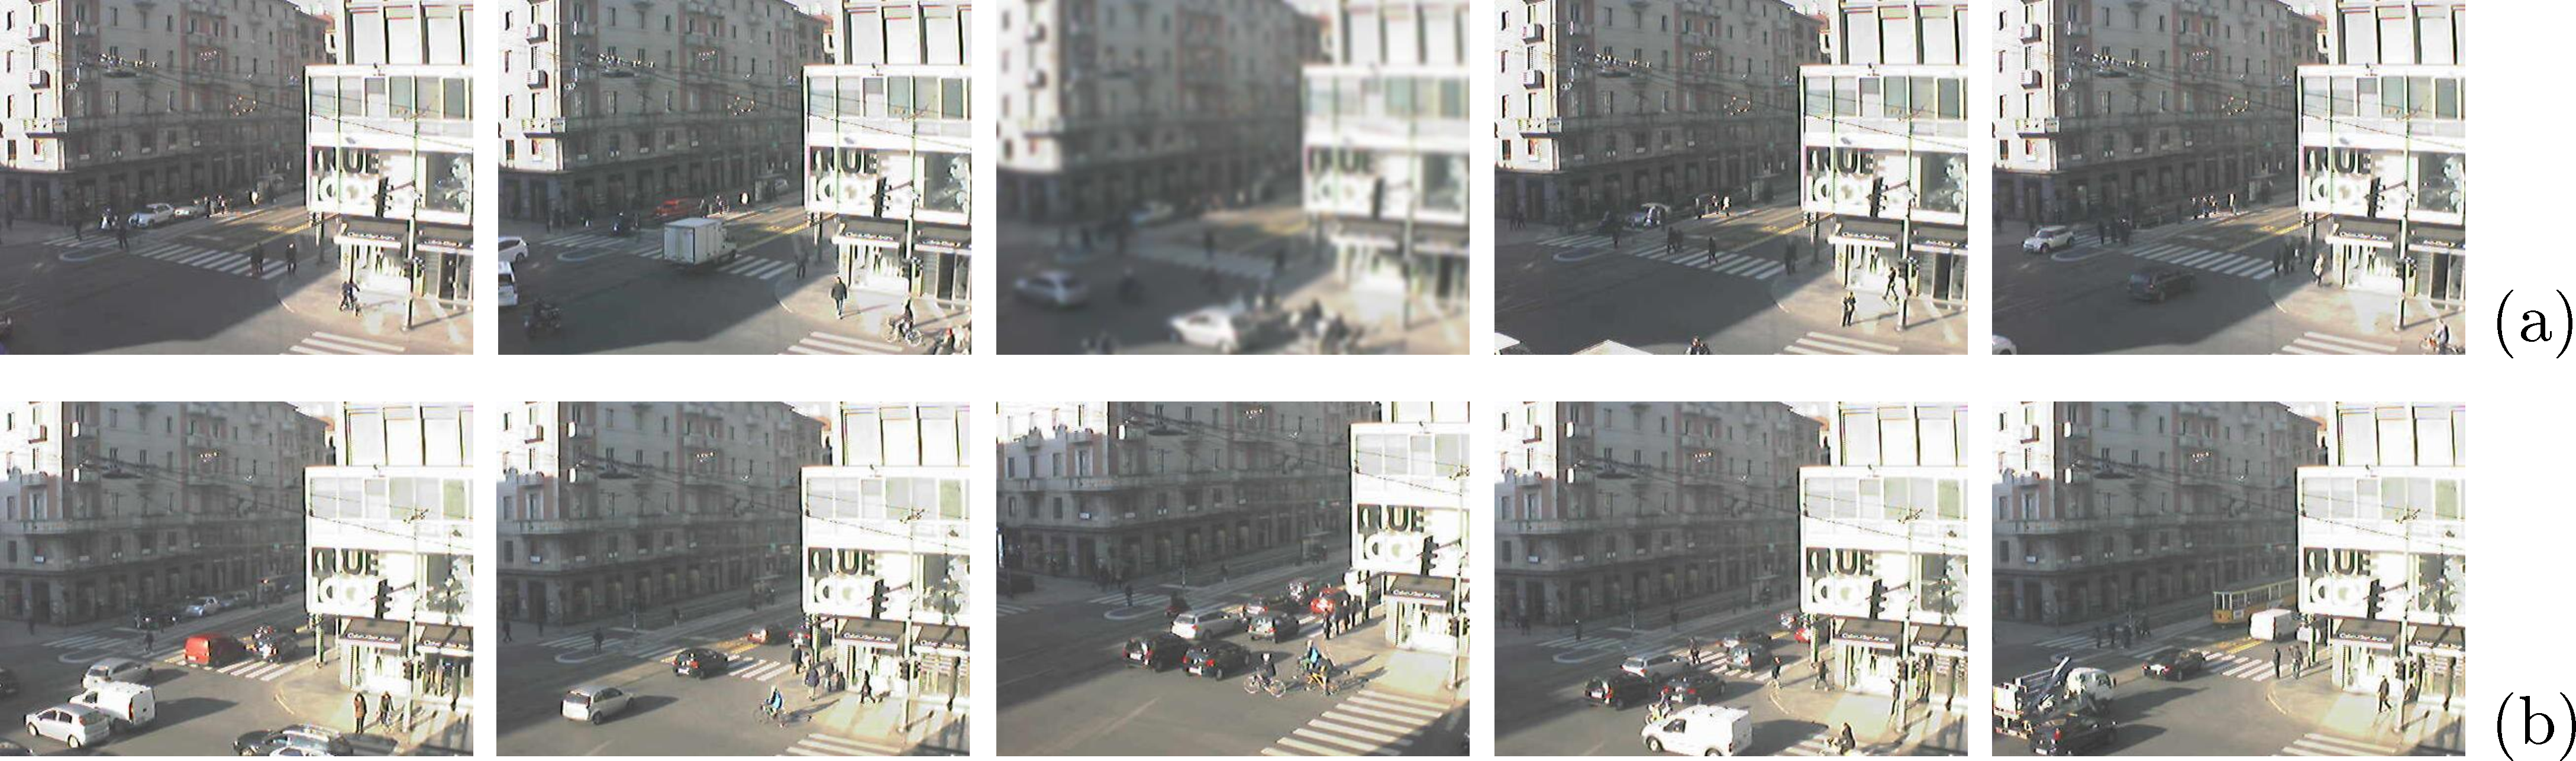
\includegraphics[width=1\linewidth]{Immagini/sequenze}
\caption{Sequences taken from webcams: \textbf{(a)} no tampering events; \textbf{(b)} defocus event on 4-th and 5-th frames, created using gaussian filtering; \textbf{(c)} displacement event on 4-th and 5-th frames, created using concatenation between similar sequences; \textbf{(d)} real displacement event on 4-th frame.}
\label{fig:sequences}
\end{figure}
The second dataset was taken using a Raspberry Pi Model B+, with its camera module, and the tampering was introduced by moving the device or putting water on the camera.\\
Four figures of merit have been suggested to assess the performance of the proposed algorithm:\\
\begin{description}
	\item[TP]  True positives. It measures the number of tampering events correctly detected by the algorithm.\\ 
	\item[TN]  True negatives. It measures the number of frames without tampering that are not detected by the algorithm. \\ 
	\item[FP]  False positives. It measures the number of tampering events erroneously detected by the algorithm.\\ 
	\item[FN]  False negatives. It measures the number of tampering events not detected by the algorithm. \\ 
\end{description} 
These indicators are computed varying the parameter $\gamma$, which defines the thresholds for the one-shot monitoring. 
This permits us to generate \textit{ROC curves}, where on the x-axis there is:
\[1-\text{SPECIFICITY}_\gamma = 1-\frac{\text{TN}_\gamma}{\text{TN}_\gamma+\text{FP}_\gamma}=\frac{\text{FP}_\gamma}{\text{TN}_\gamma+\text{FP}_\gamma},\]
while on th y-axis there is:
\[\text{RECALL}_\gamma=\frac{\text{TP}_\gamma}{\text{TP}_\gamma+\text{FN}_\gamma}.\]
The construction of these curves permits us to make a comparison with respect to other methods.
In particular the alternative approaches that we have considered working:
\begin{itemize}
\item considering the whole scene for the features computation;
\item considering adaptive region, as described in Section \ref{sec:propSol}, for the feature computation;
\item considering voronoi regions \cite{aurenhammer1991voronoi}, which are easier to compute with respect to our solution but don't consider the scene content, for the feature computation.
\end{itemize}

FRAME DIFFERENCE:
\begin{equation}
	\label{eq:frameDiffReg}
	\varphi^k(t) = \frac{\sum_{x \in R_k}(z_t(x) - z_{t-1}(x))^2}{|R_k|}, k=1,\dots,K.
\end{equation}

%
%% \subsection{Alternative Approaches}\label{subsec:AlternativeApproaches}
%
%
%\subsection{Performance Assessment}
%\gi{Adriano: Dire come vengono calcolate le ROC curves TPR e FPR, le cifre di merito insomma, spiegando bene che parametro varia}
%
%\gi{Adriano: metti entrambe le ROC curves, affiancate e per bene ed alcuni esempi di sequenze}
\begin{figure}[htb]
\centering
\subfigure[]{\label{fig:ROCdisplacement_luma}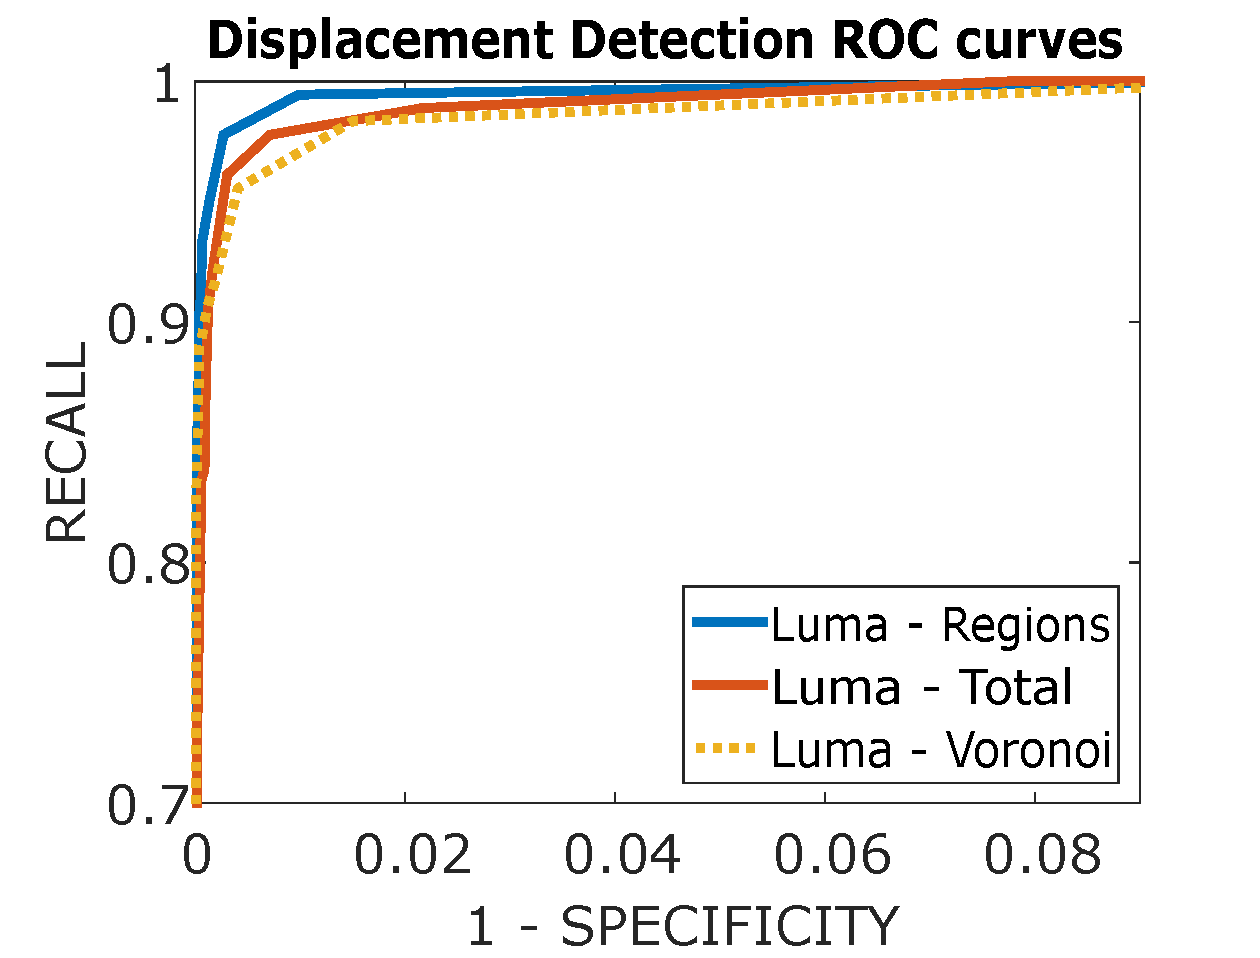
\includegraphics[width=0.45\linewidth]{Immagini/ROCdisplacement_luma}}
\subfigure[]{\label{fig:ROCdisplacement_fd} 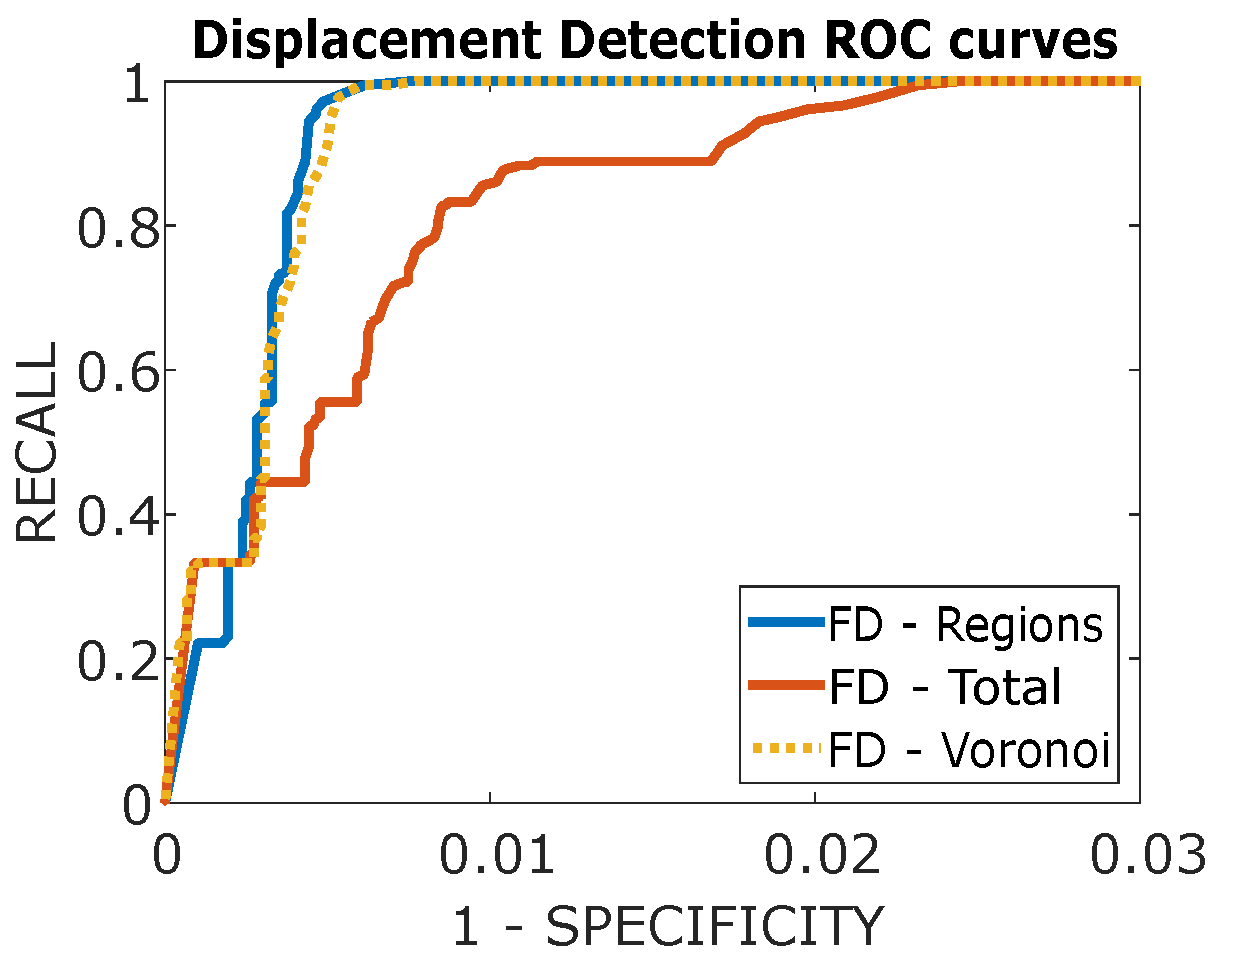
\includegraphics[width=0.45\linewidth]{Immagini/ROCdisplacement_fd}}
\caption{ROC curves for displacement detection, considering three alternative approaches. \textbf{(a)} Analysis of the mean luma energy. \textbf{(b)} Analysis of the frame differencing.}
\label{fig:ROCdisplacement}
\end{figure}
\begin{figure}[htb]
\centering
\subfigure[]{\label{fig:buenosAiresDef}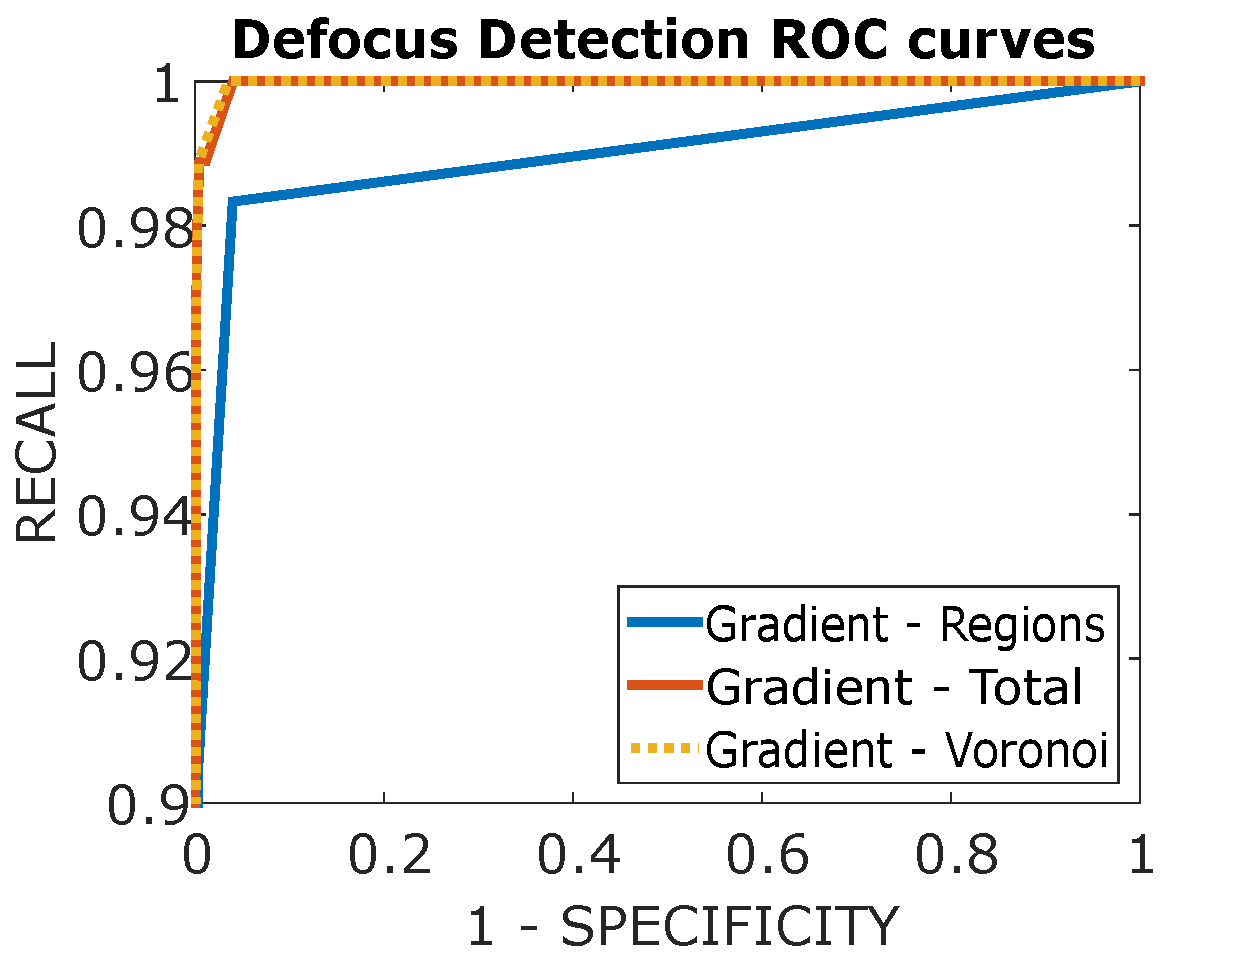
\includegraphics[width=0.45\linewidth]{Immagini/ROCdefocus1}}
\subfigure[]{\label{fig:buenosAiresDispl} 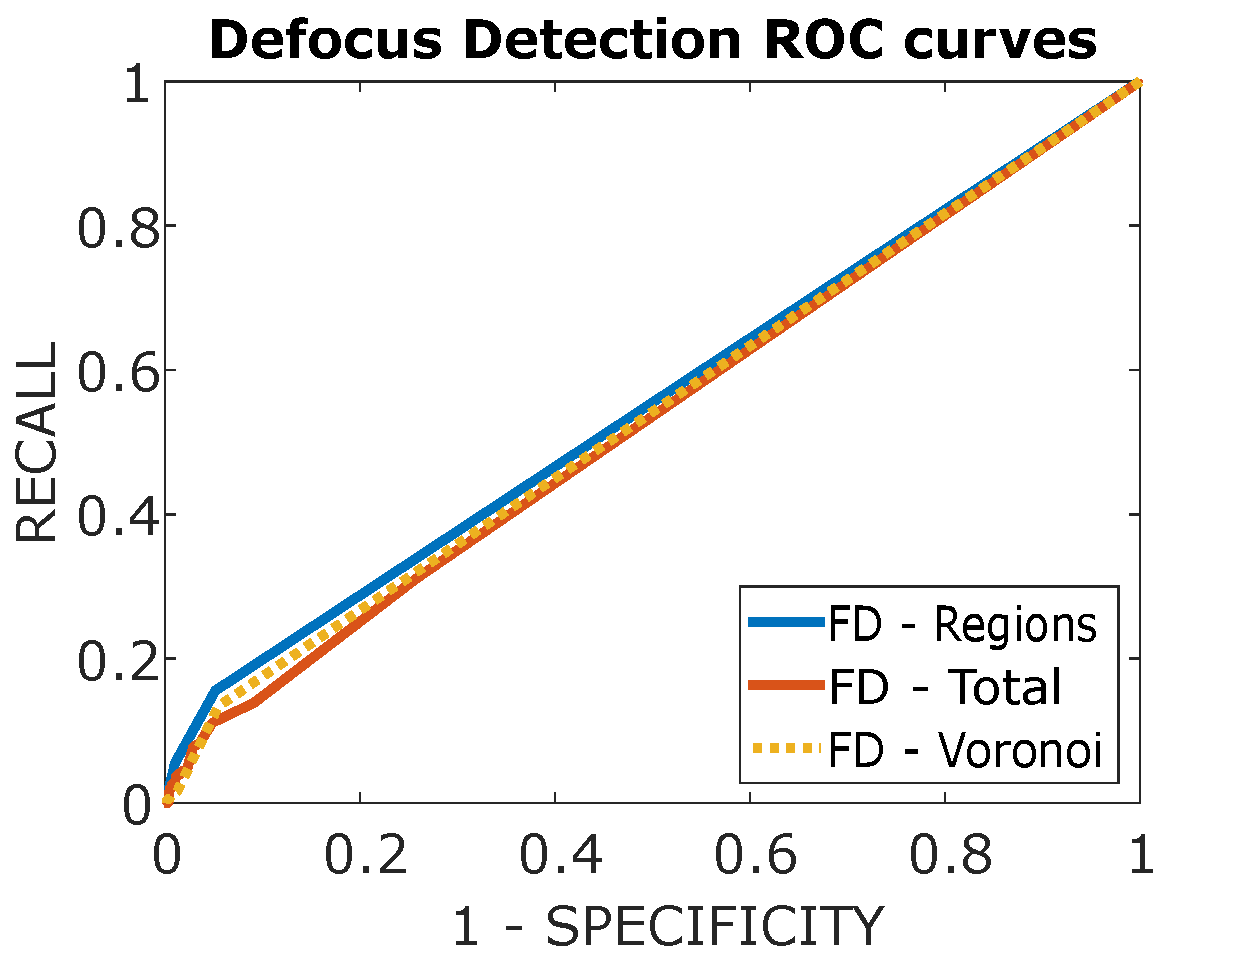
\includegraphics[width=0.45\linewidth]{Immagini/ROCdefocus_fd}}
\caption{ROC curves for defocus detection, considering three alternative approaches. \textbf{(a)} Analysis of the mean gradient energy. \textbf{(b)} Analysis of the frame differencing.}
\label{fig:ROCdisplacement}
\label{fig:ROCdefocus}
\end{figure}
Experimental results are shown in Figures \ref{fig:ROCdisplacement} and \ref{fig:ROCdefocus}.
As we could see there is an improvement, in the detection of camera displacements, with our approach which separately analizes the behavior of indicators in adaptive regions.
On the other side, as illustrated in Figure \ref{fig:ROCdefocus}, when monitoring indicators meant to detect blur/defocus, it is more convenient to consider the whole scene at once.
\subsection{Discussion}
\gi{Adriano: Aggiungi qua la complessit\'a computazionale}
% Please add the following required packages to your document preamble:
% \usepackage[table,xcdraw]{xcolor}
% If you use beamer only pass "xcolor=table" option, i.e. \documentclass[xcolor=table]{beamer}
\begin{table}[tbh]
\centering
\begin{tabular}{l|l|l|l|l|l|l|}
\cline{2-7}
& \multicolumn{3}{l|}{\cellcolor[HTML]{C0C0C0}\textbf{Displacement Detection}}  & \multicolumn{3}{l|}{\cellcolor[HTML]{C0C0C0}\textbf{Defocus Detection}} \\ \cline{2-7} 
& \cellcolor[HTML]{EFEFEF}\textbf{Regions} & \cellcolor[HTML]{EFEFEF}\textbf{Total} & \cellcolor[HTML]{EFEFEF}\textbf{Voronoi} & \cellcolor[HTML]{EFEFEF}\textbf{Regions} & \cellcolor[HTML]{EFEFEF}\textbf{Total} & \cellcolor[HTML]{EFEFEF}\textbf{Voronoi} \\ \hline
\multicolumn{1}{|l|}{\cellcolor[HTML]{EFEFEF}\textbf{Luma}}     & 0.9994 & 0.9989 & 0.9985  &            &            &             \\ \hline
\multicolumn{1}{|l|}{\cellcolor[HTML]{EFEFEF}\textbf{Gradient}} &  		 &  		  &             & 0.9895 & 0.9996 & 0.9996  \\ \hline
\multicolumn{1}{|l|}{\cellcolor[HTML]{EFEFEF}\textbf{FD}}         & 0.9974 & 0.9944 & 0.9974  & 0.5526 & 0.5322 & 0.5391  \\ \hline
\end{tabular}
\caption{Area under curve of the analized solutions}
\label{tab:AUC}
\end{table}

The algorithm uses low computational techniques: the biggest effort is made by computation of the feature $g(t)$, which needs $34$ operations per pixel, due to the Sobel filter used during the convolution.

%Numero di operazioni richieste:
%Calcolo di g(t):
%\begin{itemize}
%\item Norma gradiente: 34 FLOP per pixel
%\item Media delle norme del gradiente
%\end{itemize}
%Calcolo di l(t):
%\begin{itemize}
%\item Media dei valori di grigio
%\item Detrending: 1 FLOP per frame
%\end{itemize}
%Monitoraggio one-shot: 2 confronti
%Monitoraggio sequenziale: 
%Ogni 20 frame
%Calcolo intervalli di confidenza: ~70 FLOP
%Confronto tra intervalli di confidenza: 2 confronti



\section{Conclusion}\label{sec:Conclusion}
\gi{Adriano: butta in inglese gli ongoing works (come ultima cosa)}
.

Random Toughs:
\begin{itemize}
\item The problem of false alarms, radio module activation
\item Other tampering attacks like obfuscation (??) which might be due to environmental phenomena such as rain, fog and mist over the camera lenses have to be detected by image analysis methods
\item Displacement can be perceived by MEMS as well but these device alone are prone to false alarms. Visual inspection is necessary to reduce false alarms
\end{itemize}
Ongoing work regards the extension of our solution to other types of tampering, as occlusions or imaging sensor degradations.
Furthermore, we are investigating strategies to improve the detection performance and reduce the number of \textit{FP}s by combination of our solution with other techniques:
for example we could use sequential techniques on the features, or integrate the frame analysis with the data extracted from MEMS inertial sensors.   

\section*{Acknowledgments}\label{sec:Acknowledgments}
Authors would like to thank ST for supporting Adriano Gaibotti.

\bibliographystyle{unsrt}
\bibliography{bibl_tesi}

%\begin{thebibliography}{1}
%	
%	\bibitem{Einstein}
%	A. Einstein, On the movement of small particles suspended in stationary liquids required by the molecular-kinetic theory of heat, Annalen der Physik 17, pp. 549-560, 1905.
%	
%\end{thebibliography}
\end{document}



%
%
%
\subsection{Indicators}\label{subsec:Indicators}

%\begin{equation}
%\label{eq:gradientRegions}
%\begin{array}{ccc}
%g^k(t)&  = & \mathcal{G}^k[z_t] = \frac{\sum_{R_k}\| \nabla z_t(x) \| _2^2 }{|{R_k}|}\\
%\partial g^k(t) & =& g^k(t)-g^k(t-1) 
%\end{array},
%\end{equation}
%
%In particolare, per il calcolo delle derivate orizzontali  abbiamo utilizzato il seguente filtro $f_h$:
%\[f_h = f \circledast \left[ \begin{array}{rcl}
%1 & 0 & -1
%\end{array}\right], \] 
%mentre per il calcolo delle derivate verticali abbiamo utilizzato il seguente filtro $f_v$:
%\[f_v = f \circledast \left[ \begin{array}{r}
%1 \\ 0 \\ -1
%\end{array}\right], \]
%dove abbiamo indicato con $\circledast$ l'operatore di convoluzione.
%Il filtro $f$, invece, \`e ottenuto tramite un campionamento della \textit{funzione gaussiana} $h$, con media $0$ e deviazione standard $\sigma$
%\begin{equation}
%\label{eq:gaussian}
%h(i,j)=\frac{1}{2\pi\sigma^2}\exp\left(-\frac{i^2+j^2}{2\sigma^2}\right),
%\end{equation}
%e ponendo il valore massimo di questa funzione nel centro del filtro.
%Con questi filtri \`e possibile calcolare la \textit{norma del gradiente} nel seguente modo:
%
%Una volta calcolata la norma del gradiente \`e possibile farne la media come specificato in \eqref{eq:energyGradient}.
%Il risultato finale \`e un indicatore \textit{scalare} per ciascun frame acquisito, che pu\`o essere monitorato per individuare eventi di sfocature. 
%In particolare ci aspettiamo che l'evento di sfocatura provochi un abbattimento del valore di $g$.